% ------------------------------------------------------------------------------
% TYPO3 CMS 7.3 - What's New - Chapter "Introduction" (English Version)
%
% @author	Michael Schams <schams.net>
% @license	Creative Commons BY-NC-SA 3.0
% @link		http://typo3.org/download/release-notes/whats-new/
% @language	English
% ------------------------------------------------------------------------------
% LTXE-CHAPTER-UID:		066dde91-8cd613b5-0eadb76c-a6245b74
% LTXE-CHAPTER-NAME:	Introduction
% ------------------------------------------------------------------------------

\section{Introducción}
\begin{frame}[fragile]
	\frametitle{Introducción}

	\begin{center}\huge{Introducción}\end{center}
	\begin{center}\huge{\color{typo3darkgrey}\textbf{Los Hechos}}\end{center}

\end{frame}

% ------------------------------------------------------------------------------
% LTXE-SLIDE-START
% LTXE-SLIDE-UID:		5f14b3ab-7a637a25-94057423-a1600ba3
% LTXE-SLIDE-ORIGIN:	1c3389b6-2103f93f-b2319a3e-aacc6eba English
% LTXE-SLIDE-ORIGIN:	6d5e9f3e-f9d9677e-43d7d497-e80ba9ef German
% LTXE-SLIDE-TITLE:		TYPO3 CMS 7.3 - The Facts
% ------------------------------------------------------------------------------
\begin{frame}[fragile]
	\frametitle{Introducción}
	\framesubtitle{TYPO3 CMS 7.3 - Los Hechos}

	\begin{itemize}
		\item Fecha de lanzamiento: 16 de Junio 2015
		\item Tipo de lanzamiento: "Lanzamiento Sprint"
		\item Visión: Adoptar, Innovar, Lanzar
		\item Foco principal: Ecosistema de Paquetes, Composer y Manejo de Extensiones
	\end{itemize}

\end{frame}

% ------------------------------------------------------------------------------
% LTXE-SLIDE-START
% LTXE-SLIDE-UID:		0075ce46-8e68d24c-2a4f3b7c-cb564c4c
% LTXE-SLIDE-ORIGIN:	780b1e6f-e761ec98-824890a3-8d429b56 English
% LTXE-SLIDE-ORIGIN:	759c3860-d5061f6e-2bb0009f-6ea130c8 German
% LTXE-SLIDE-TITLE:		System Requirements
% ------------------------------------------------------------------------------
\begin{frame}[fragile]
	\frametitle{Introducción}
	\framesubtitle{Requisitos del Sistema}

	\begin{itemize}
		\item PHP*:\tabto{2.2cm}v5.5.0 - v5.6.x
		\item MySQL:\tabto{2.2cm}v5.5.x - v5.6.x (modo no estricto)
		\item Espacio de disco:\tabto{3.4cm}min 200 MB
		\item Ajustes de PHP:

			\begin{itemize}
				\item memory\_limit >= 128M
				\item max\_execution\_time >= 240s
				\item opción de compilación \texttt{--disable-ipv6} \underline{no} debe ser usada
			\end{itemize}

		\item Backend requiere IE >= 9 o cualquier otro navegador moderno

	\end{itemize}

	\vspace{1cm}
	*) Detalles adicionales: \href{http://typo3.org/news/article/php-minimum-requirements-for-typo3-cms-7/}{Requisitos Mínimos de PHP para TYPO3 CMS 7}

\end{frame}

% ------------------------------------------------------------------------------
% LTXE-SLIDE-START
% LTXE-SLIDE-UID:		32ee4fc9-acb8e2e8-5a918734-5253f555
% LTXE-SLIDE-ORIGIN:	e06c97c6-ee283664-40fe3fe5-af3a1caa English
% LTXE-SLIDE-ORIGIN:	70c77c41-e2b83d82-2f182996-98061070 German
% LTXE-SLIDE-TITLE:		Development And Release Timeline
% ------------------------------------------------------------------------------
\begin{frame}[fragile]
	\frametitle{Introducción}
	\framesubtitle{Línea de tiempo de Desarrollo y Lanzamiento}

	\begin{figure}
		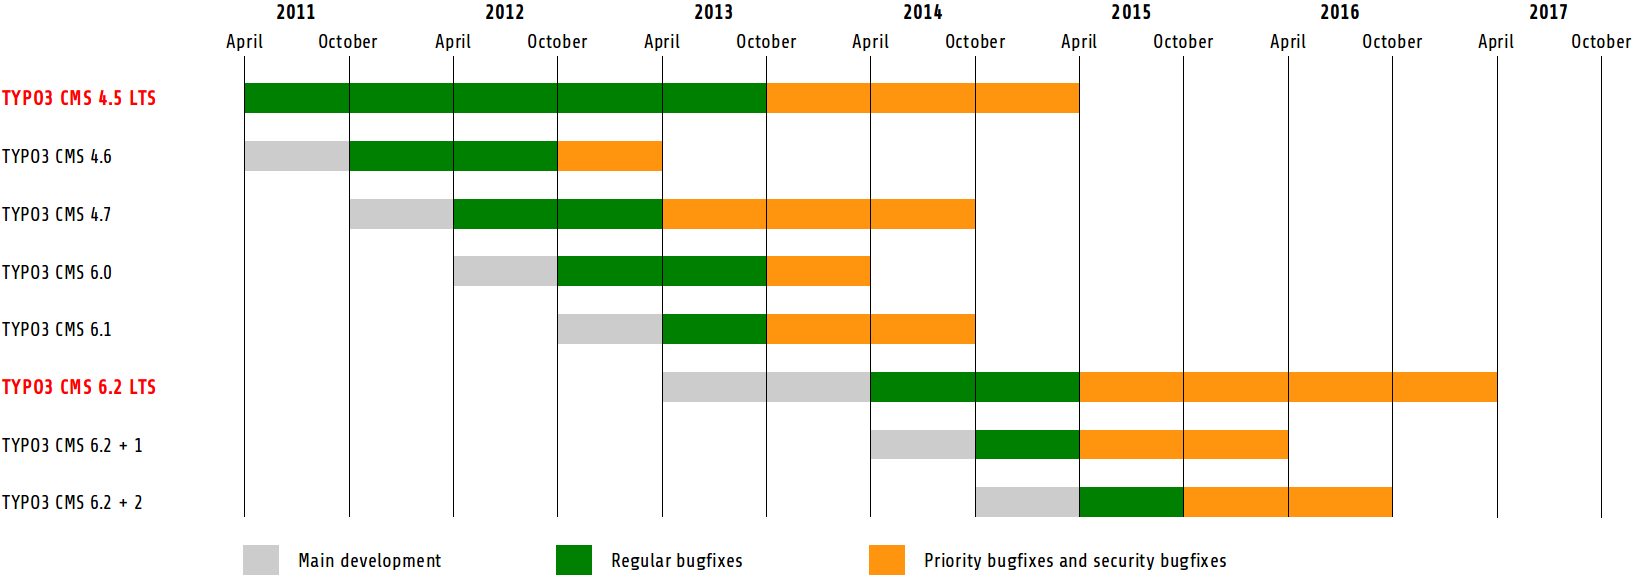
\includegraphics[width=0.90\linewidth]{Introduction/ReleaseAgenda.png}
	\end{figure}

\end{frame}

% ------------------------------------------------------------------------------
% LTXE-SLIDE-START
% LTXE-SLIDE-UID:		1774290d-367cd978-14d42099-9a40cdd2
% LTXE-SLIDE-ORIGIN:	cfdf68b1-b00a3fca-0adf0630-7563d7da English
% LTXE-SLIDE-ORIGIN:	b55d3fe9-76807061-d97f3fee-7db1f190 German
% LTXE-SLIDE-TITLE:		TYPO3 CMS Roadmap
% ------------------------------------------------------------------------------
\begin{frame}[fragile]
	\frametitle{Introducción}
	\framesubtitle{Línea de lanzamiento de TYPO3 CMS}

	Fechas de lanzamiento estimadas y sus enfoques principales:

	\begin{itemize}
		\item v7.0 \tabto{1.0cm}02/Dic/2014\tabto{3.4cm}Revisión de Backend Vol 1
		\item v7.1 \tabto{1.0cm}24/Feb/2015\tabto{3.4cm}Optimización \& Limpieza del núcleo
		\item v7.2 \tabto{1.0cm}28/Apr/2015\tabto{3.4cm}Frontend

		\item
			\begingroup
				\color{typo3orange}
					v7.3 \tabto{1.0cm}16/Jun/2015\tabto{3.4cm}Ecosistema de Paquetes, Composer\newline
					\tabto{3.4cm}y Manejo de Extensiones
			\endgroup

		\item v7.4 \tabto{1.0cm}04/Ago/2015\tabto{3.4cm}Revisión de Backend Vol 2
		\item v7.5 \tabto{1.0cm}29/Sep/2015\tabto{3.4cm}\textit{(por determinar...)}
		\item v7.6 \tabto{1.0cm}xx/xxx/2015\tabto{3.4cm}\textbf{TYPO3 CMS 7 LTS} (Soporte a Largo Plazo)
	\end{itemize}

	\smaller
		\url{https://typo3.org/typo3-cms/roadmap/}\newline
		\url{http://typo3.org/news/article/embrace-and-innovate-typo3-cms-7/}
	\normalsize

\end{frame}

% ------------------------------------------------------------------------------
% LTXE-SLIDE-START
% LTXE-SLIDE-UID:		35aa2e44-cef721ca-3b32ab2d-79fcd0c6
% LTXE-SLIDE-ORIGIN:	eb02037c-0fba04b6-5006d3f3-03fe223a English
% LTXE-SLIDE-ORIGIN:	b0c28f26-c3ca2e99-195954a8-ed76f9d4 German
% LTXE-SLIDE-TITLE:		Installation
% ------------------------------------------------------------------------------
\begin{frame}[fragile]
	\frametitle{Introducción}
	\framesubtitle{Instalación}

	\begin{itemize}
		\item Procedimiento de instalación oficial bajo Linux/Mac OS X\newline
			(DocumentRoot por ejemplo \texttt{/var/www/site/htdocs}):
		\begin{lstlisting}
			$ cd /var/www/site
			$ wget --content-disposition get.typo3.org/7.3
			$ tar xzf typo3_src-7.3.0.tar.gz
			$ cd htdocs
			$ ln -s ../typo3_src-7.3.0 typo3_src
			$ ln -s typo3_src/index.php
			$ ln -s typo3_src/typo3
			$ touch FIRST_INSTALL
		\end{lstlisting}

		\item Enlaces simbólicos bajo Microsoft Windows:

			\begin{itemize}
				\item Use \texttt{junction} en Windows XP/2000
				\item Use \texttt{mlink} en Windows Vista y Windows 7
			\end{itemize}

	\end{itemize}
\end{frame}

% ------------------------------------------------------------------------------
% LTXE-SLIDE-START
% LTXE-SLIDE-UID:		c83cccff-7d4e2f32-faa7d5f8-21b7f38a
% LTXE-SLIDE-ORIGIN:	5c2e0134-2f1f18d2-55b74162-25dd3995 English
% LTXE-SLIDE-ORIGIN:	48136734-ae508d23-bce5811d-667f8908 German
% LTXE-SLIDE-TITLE:		Upgrade to TYPO3 CMS 7
% ------------------------------------------------------------------------------
\begin{frame}[fragile]
	\frametitle{Introducción}
	\framesubtitle{Actualización a TYPO3 CMS 7.x}

	\begin{itemize}
		\item Actualizaciones sólo posibles desde TYPO3 CMS 6.2 LTS
		\item TYPO3 CMS < 6.2 deberá ser actualizado a TYPO3 CMS 6.2 LTS primero
	\end{itemize}

	\begin{itemize}

		\item Instrucciones de actualización:\newline
			\smaller\url{http://wiki.typo3.org/Upgrade#Upgrading_to_7.3}\normalsize
		\item Guía oficial de TYPO3 "Instalación y Actualización de TYPO3":
			\smaller\url{http://docs.typo3.org/typo3cms/InstallationGuide}\normalsize
		\item Enfoque general:
			\begin{itemize}
				\item Comprobar requisitos mínimos del sistema \small(PHP, MySQL, etc.)
				\item Revisar \textbf{deprecation\_*.log} en instancia antigua de TYPO3
				\item Actualizar todas las extensiones a las últimas versiones
				\item Desplegar fuentes nuevas y ejecutar Herramienta de Instalación \textrightarrow Asistente de Actualización
				\item Revisar el módulo de inicio para usuarios backend (opcionalmente)
			\end{itemize}
	\end{itemize}

\end{frame}

% ------------------------------------------------------------------------------
